\documentclass{beamer}


\usepackage{graphicx}
\usepackage{amsmath}
\usepackage{mathdots}
\usepackage{amsthm}
\usepackage{amssymb}
\usepackage{pstricks}
\usepackage{pst-node}
\pagenumbering{arabic}
\usepackage{hyperref}
\usepackage{lscape}
\usenavigationsymbolstemplate{}
\definecolor{slidetitlecolor}{RGB}{51,0,102}
\setbeamertemplate{footline}[frame number]%puts frame numbers in slide
\setbeamercolor{frametitle}{fg=slidetitlecolor}
\definecolor{item1color}{RGB}{51,153,255}
\setbeamercolor{itemize item}{fg=item1color}
\setbeamertemplate{itemize item}[circle]
\setbeamercolor{enumerate item}{fg=item1color}

\title{Queueing Theory\vspace{-.5cm}}
\author{VK\\
Room: M1.30\\
knightva@cf.ac.uk\\
www.vincent-knight.com}
\date{\tiny{Last updated: \today.}}




\begin{document}

\maketitle


\frame{\frametitle{Overview}\tableofcontents}
\section{Description of Queueing Processes}
\frame{\frametitle{Description of Queueing Processes}}
\frame{\frametitle{Queueing Theory}
A queueing system consists of:
\begin{center}
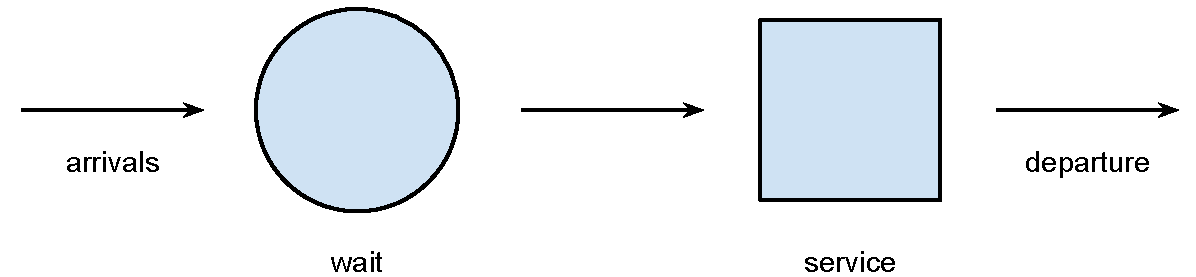
\includegraphics[width=7cm]{Queueing_Process.pdf}
\end{center}
\begin{itemize}
\item Arrival process
\item Waiting regime
\item Service process
\item Departure process
\end{itemize}
}

\frame{\frametitle{Examples}
\begin{itemize}
\item Customers waiting to pay at the supermarket
\item Patients at a medical clinic waiting to see a doctor
\item Passengers waiting at the bus stop
\item Aeroplanes circling an airport waiting to land
\item Parts on a production line waiting for further processing
\end{itemize}
}

\frame{\frametitle{Arrival Process}
The arrival process can be:
\begin{itemize}
\item Deterministic:
\begin{center}
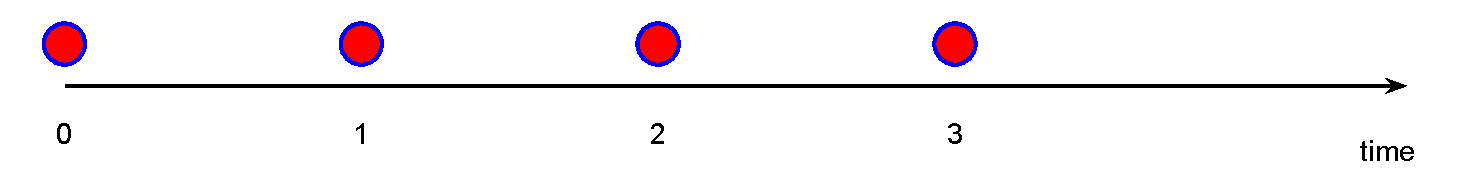
\includegraphics[width=7cm]{Deterministic_Arrival_Process.pdf}
\end{center}
\item Random:
\begin{center}
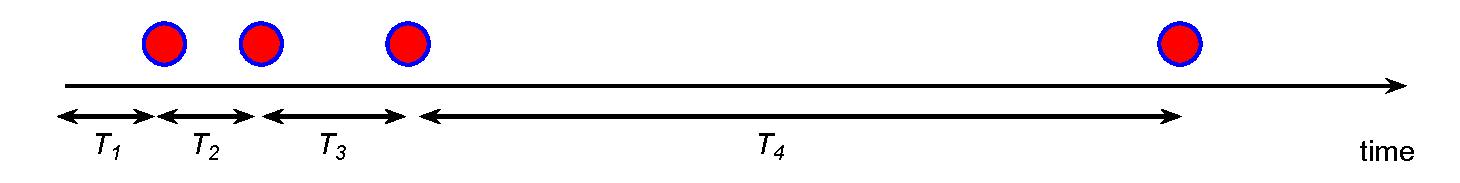
\includegraphics[width=7cm]{Random_Arrival_Process.pdf}
\end{center}
Here $T_1,T_2,T_3,\dots$ are random \emph{interarrival} times.
\end{itemize}
}

\frame{\frametitle{Arrival Process}
\begin{itemize}
\item Batched:
\begin{center}
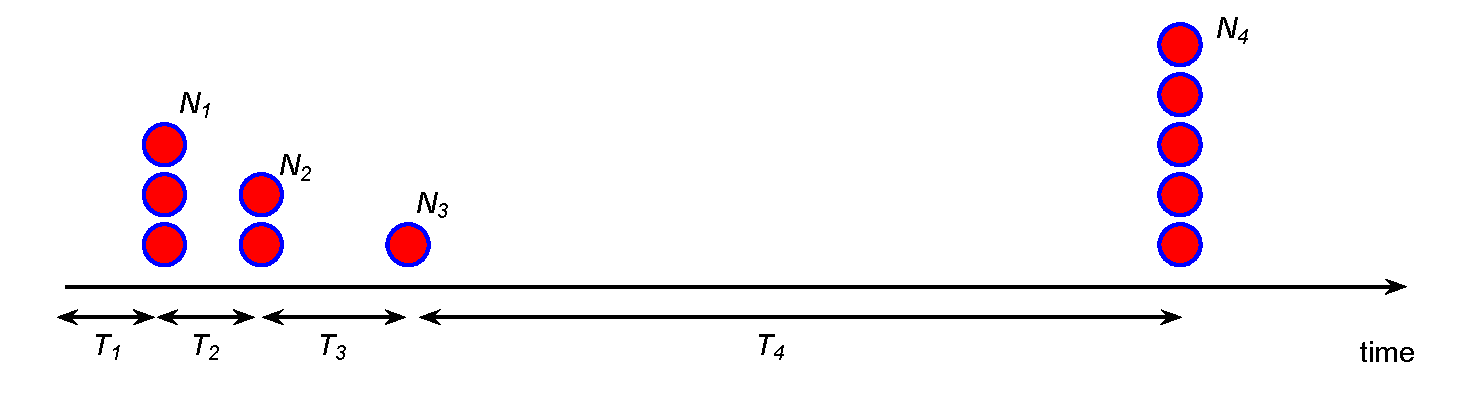
\includegraphics[width=7cm]{Batched_Arrival_Process.pdf}
\end{center}
The \emph{batch sizes} $N_i$ and \emph{interarrival} times $T_i$ can be deterministic or random.
\item Typed arrivals: arrivals can be of different types, requiring different types of service.
\end{itemize}
We consider random arrivals on this course.
}

\frame{\frametitle{Waiting Regime}
The waiting regime typically consists of a buffer size. This is just the maximum number of people/units that can wait in the queue to be served. People/units that arrive when the buffer is full are either lost to the system, or come back later.
}

\frame{\frametitle{Service Process}
The service process typically consists of:
\begin{itemize}
\item Service times: can be deterministic, random, batched and/or depend on the type of customer. They can also depend on the queue size.
\item Number of servers
\item The service discipline:
\begin{itemize}
\item FIFO: \textbf{F}irst \textbf{I}n \textbf{F}irst \textbf{O}out
\item LIFO: \textbf{L}ast \textbf{I}n \textbf{F}irst \textbf{O}out
\item SIRO: \textbf{S}ervice \textbf{I}n \textbf{R}andom \textbf{O}rder
\end{itemize}
\end{itemize}
}

\frame{\frametitle{Departure Process}
This is the outcome of the arrival, waiting and service processes.
}

\frame{\frametitle{Examples}
\begin{itemize}
\item Customer waiting to pay at the supermarket. Random arrivals. Multiple servers with random service times, number may depend on queue size. May have typed customers such as ``8 items of less'' or ``pay by cash'',
\item Patients at a medical clinic waiting to see a doctor. Deterministic arrivals (appointment times). Random service times.
\item Passengers waiting at the bus stop. Random arrivals. Random service times with batched service.
\item Aeroplanes circling an airport waiting to land. Random arrivals. Deterministic service times (approximately every 2 minutes at Heathrow).
\end{itemize}
}
\frame{\frametitle{Aims of queueing analysis}}
\frame{\frametitle{Aims of queueing analysis}
In general we want to know things like:
\begin{itemize}
\item Average time a customer is in the system
\item Average queue length
\item Utilisation of servers (proportion of time busy)
\end{itemize}
These are examples of \emph{performance measures} for the system. We may be designing or trying to improve a queueing system. We would like to be able to gauge the effect of:
\begin{itemize}
\item A change in arrival rate
\item A change in service time
\item A change in the number of servers
\item A change in the service regime
\end{itemize}
}

\frame{\frametitle{Approaches to queueing analysis}
There are a variety of approaches to the study of queueing systems:
\begin{itemize}
\item \textbf{Real World:} real-world systems provide the best information, but are expensive to experiment with.
\item \textbf{Simulation:} simulation allows cheap analysis of the effects of change to a system and is the only practical way to deal with very complex queueing systems.
\item \textbf{Theory:} theoretical analysis is only possible for relatively simple systems, but provides unrivalled insight into why queues behave as they do,
\end{itemize}
This course takes the theoretical approach to queueing.
}

\frame{\frametitle{Example}
Suppose 3 customers arrive one just after the other with service requirements (in units of time):
$$10,20,30$$
In a FIFO regime the average time in the system will be:
$${10+30+60\over 3}={100\over3}$$
In a LIFO regime the average time in the system will be:
$${30+50+60\over 3}={140\over3}$$
}

\frame{\frametitle{The arrival process}
The most important characteristic of the arrival process is:
$$\lambda=\text{ average number of arrivals per unit time}$$
Note that $\lambda$ depends on the time unit you use, so that $\lambda=2$ arrivals per \textbf{minute} is equivalent to $\lambda=120$ arrivals per \textbf{hour}.\\\vspace{.5cm}
The arrival rate can change over time, in which case we use the notation $\lambda(t)$ for the arrival rate at time $t$.\\\vspace{.5cm}
We assume that arrivals follow a Poisson process for the rest of the course.
}

\frame{\frametitle{The arrival process}
If an arrival process is a Poisson process, the number of arrivals occurring within any interval of time of length $t$, follows a \textbf{Poisson} distribution with parameter $\lambda t$.\\\vspace{.5cm}
The probability that there are $n$ arrivals in a time interval of length $t$ is equal to:
$$p(n)={(\lambda t)^ne^{-\lambda t}\over n! }\text{ for }n=0,1,2,\dots$$
and is independent of the number of units currently in the system or the history of arrivals prior to the start of the interval.\\\vspace{.5cm}
The average number of arrivals in an interval of length $t$ is $\lambda t$ and the variance is also equal to $\lambda t$ (properties of the Poisson distribution).
}

\frame{\frametitle{Infinitesimal Arrival Rate}
Consider a short interval of length $\gamma t$ and let $N(t,t+\gamma t)$ be the number of arrivals between $t$ and $t+\gamma t$. From the expression for the Poisson distribution:
$$P(N(t,t+\gamma t)=1)=(\lambda\gamma t)e^{-\lambda\gamma t}=(\lambda\gamma t)\left(1-\lambda\gamma t+{(\lambda\gamma t)^2\over2}-\dots\right)$$
where we have expanded $e^{-\lambda\gamma t}$ in a Taylor series. As $\gamma t\to0$, $(\gamma t)^2$ and higher order terms become negligible and:
$$\begin{array}{@{}r@{\;}c@{\;}l@{}}
P(N(t,t+\gamma t)=1)&\approx&\lambda\gamma t\\[2mm]
P(N(t,t+\gamma t)=0)&\approx&1-\lambda\gamma t\\[2mm]
P(N(t,t+\gamma t)>1)&\approx&0
\end{array}$$
}

\frame{\frametitle{Inter-Arrival Times}
For a poisson process, the time between events (arrivals) must follow a negative exponential distribution. \\\vspace{.5cm}
To show this, assume we start observing a Poisson process immediately after an event (arrival) and say this occurred at time $0$. The probability that we have no events at time $t$ is:
$$P(N(0,t)=0)=e^{-\lambda t}$$
but this is equal to the probability that the time between two successive events (arrivals) is greater than $t$. Writing $X$ as the time between two successive event (arrivals), this means that:
$$\begin{array}{@{}r@{\;}c@{\;}l@{}}
P(X>t)&=&e^{-\lambda t}\\[2mm]
P(X\leq t)&=&1-e^{-\lambda t}
\end{array}$$
}

\frame{\frametitle{Inter-Arrival Times}
We know that $P(X\leq t)=F(t)$, where $F(t)$ is the \textbf{cumulative density function} (cdf) of the distribution of time between events. The \textbf{probability density function} (pdf) is given by
$$\begin{array}{@{}r@{\;}c@{\;}l@{}}
f(t)&=&{dF(t)\over dt}\\[2mm]
f(t)&=&\lambda e^{-\lambda t}
\end{array}$$
but this is the pdf of a negative exponential distribution. Thus, inter arrival times $\sim NegExp(\lambda)$.
}

\frame{\frametitle{The memoryless property}
The most important property of the negative exponential distribution is the memoryless property. This says that \emph{if you have a $NegExp(\lambda)$ inter arrival time, and have already waited time $t$ for the next arrival, then the time remaining until the next arrival still have $NegExp(\lambda)$ distribution.}\\\vspace{.5cm}
i.e. the amount of time you have waited tells you nothing about how long you still have to wait.\\\vspace{.5cm}
The exponential distribution is the \textbf{only} continuous distribution with this property. It can be used to describe e.g. the arrival of telephone calls at an exchange, the arrival of customer at a store $\dots$
}

\frame{\frametitle{The memoryless property}
The memoryless property is equivalent to the conditional probability statement:
$$P(T_i>s+t\;|\;T_i>s)=P(T_i>t)$$
The proof is a straight forward application of the definition of conditional probability, and the fact that $P(T_i>t)=e^{-\lambda t}$:
$$\begin{array}{@{}r@{\;}c@{\;}l@{}}
P(T_i>s+t\;|\;T_i>s)&=&{P(\;T_i>s\;|T_i>s+t\;)P(\;T_i<s+t\;)\over P(T_i>s)}\\[2mm]
&=&{P(T_i>s+t)\over P(T_i>s)}\\
&=&{e^{-\lambda (s+t)}\over e^{-\lambda s}}=e^{-\lambda t}=P(T_i>t)
\end{array}$$
}

\frame{\frametitle{Memoryless property paradox}
Consider the following argument. Suppose we have a Poisson process of rate $\lambda$, and we turn up at some random time $t$ to observe it. On average, we will arrive half way between two arrivals. Thus the expected time until the next arrival will be half the expected time between any two arrivals, that is ${1\over 2\lambda}$.\\\vspace{.5cm}\pause
But the memoryless property tells us that the time from our appearance to the next arrival should still be $NegExp(\lambda)$, with mean ${1\over\lambda}$: a contradiction!
}

\frame{\frametitle{Memoryless property paradox}
Of course there is a flaw in the previous argument.\\\vspace{.5cm}
If we turn up at a random time, then we are more likely to turn up between two widely spaced arrivals than between two closely spaced arrival. Thus, the inter arrival period we turn up in will on average be larger than the norm, and so its expected length will be larger than the norm (in fact, exactly twice the norm)
}

\frame{\frametitle{Merging and thinning}
The poisson process has many useful properties. Two of these concern merging and thinning.
\begin{center}
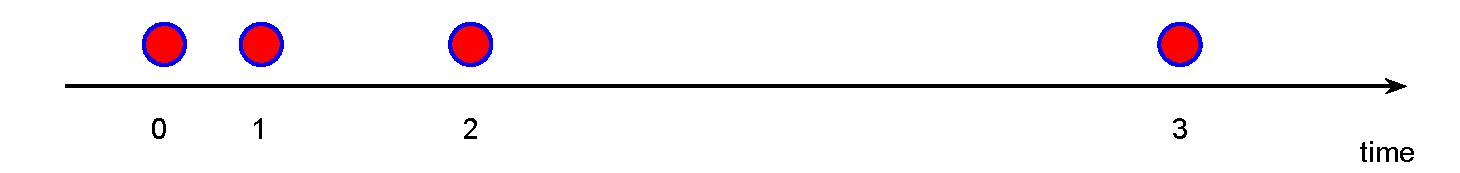
\includegraphics[width=7cm]{Merging_1.pdf}
\end{center}
$$+$$
\begin{center}
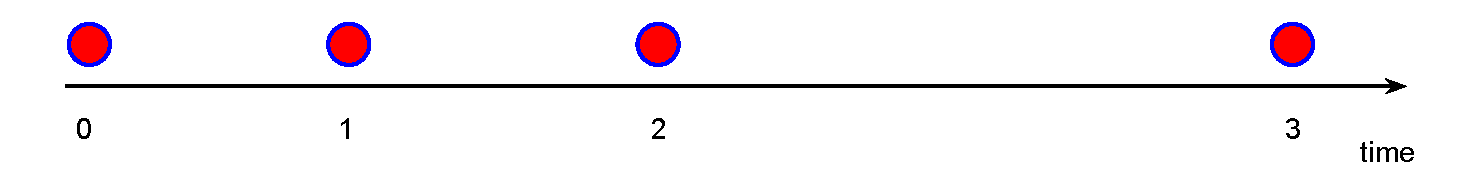
\includegraphics[width=7cm]{Merging_2.pdf}
\end{center}
$$=$$
\begin{center}
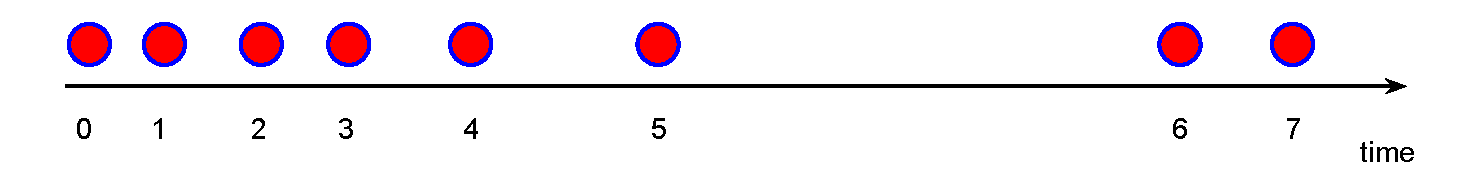
\includegraphics[width=7cm]{Merging_12.pdf}
\end{center}}

\frame{\frametitle{Merging and thinning}
If we merge a Poisson process rate $\lambda_1$ with an independent Poisson process rate $\lambda_2$, then the result is a Poisson process rate $\lambda_1+\lambda_2$. By merging we mean that we add all of the arrivals together.
}

\frame{\frametitle{Merging and thinning}
We thin a process by selecting arrivals at random. For example we could toss a coin for each arrival: heads we keep it, tails it is discarded.
\begin{center}
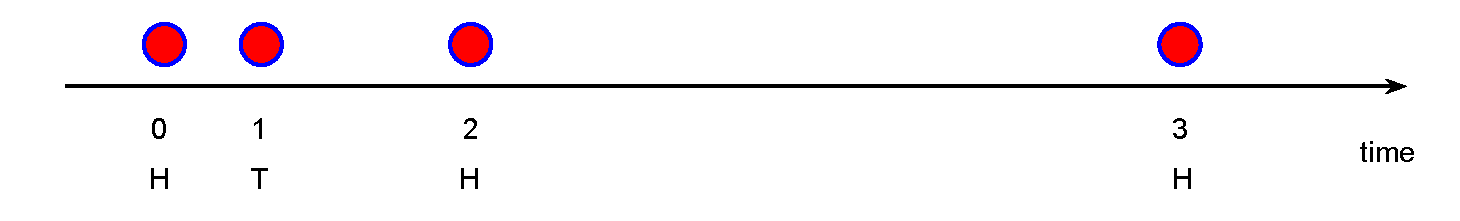
\includegraphics[width=7cm]{Thinning_1.pdf}
\end{center}\pause
\begin{center}
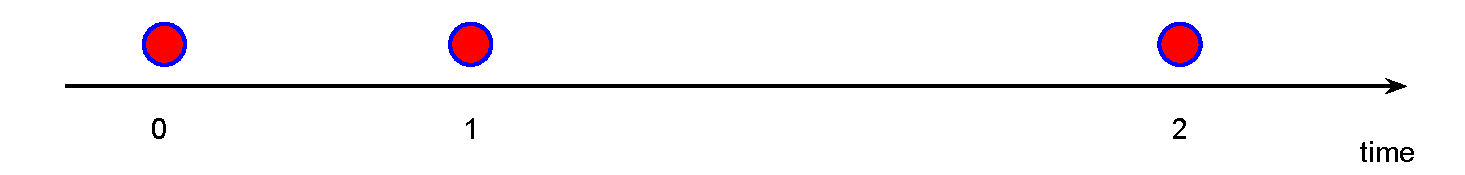
\includegraphics[width=7cm]{Thinning_2.pdf}
\end{center}
}

\frame{\frametitle{Merging and thinning}If we start with a Poisson process rate $\lambda$, and the probability of keeping an arrival is $p$, then the results is a Poisson process rate $p\lambda$.\\\vspace{.5cm} (A proof of these results is not part of the course)}


\frame{\frametitle{The service process}
Most simple queueing models assume that that service times have a negative exponential distribution with parameter $\mu$, so that the pdf is written as:
$$f(t)=\mu e^{-\mu t}$$
where ${1\over\mu}$ is the average length of a service.\\\vspace{.5cm}
If this is true, the service process is also a Poisson process and service times will also obey the memoryless property. For example, if you arrive at a cash desk and find the server busy and the service process is a Poisson process, the expected time until the service finishes serving will be independent of how long the current service has been in progress.
}

\frame{\frametitle{The service process}
What is the expected waiting time of a unit that joins the queue and finds $n$ unites ahead of it($n-1$ in the queue and 1 being served)?
$$\begin{array}{@{}r@{\;}c@{\;}l@{}}
\text{Total expected time}&=&n\times{1\over\mu}={n\over \mu}\\[2mm]
\text{Variance}&=&n\times{1\over\mu^2}={n\over \mu^2}\\
\text{Standard deviation}&=&{\sqrt{n}\over \mu}
\end{array}$$
The distribution of the waiting times is the convolution of $n$ negative exponential distributions. I.e. a gamma distribution with parameters $(n,\mu)$:
$$f(t)={\mu t^{n-1}e^{-\mu t}\over (n-1)!},\;t\geq 0$$
}

\frame{\frametitle{Classification of queues}
There is a classification scheme for commonly encountered queues (originally devised by David Kendall). A general queue is denoted:
$$A/B/m/n$$
where we make the following assumptions:
\begin{enumerate}
\item Inter-arrival times are independent and give by some distribution $A$.
\item Service times are independent and given by some distribution $B$.
\item There are $m$ servers.
\item There is a buffer of size $n$.\end{enumerate}
}

\frame{\frametitle{Standard notation for distributions}
There is also some standard notation for the possible types of distribution $A$ and $B$:
\begin{itemize}
\item $M$ the exponential distribution (Markovian)
\item $D$ deterministic
\item $E_k$ the Erlang distribution with $k$ stages
\item $H_k$ the hyper-exponential with $k$ channels
\item $G$ a general distribution
\end{itemize}
}
\section{The Single Server Markovian Queue}
\frame{\frametitle{The $M/M/1$ queue}}
\frame{\frametitle{The $M/M/1$ queue}
The $M/M/1$ queue has Markov arrival and service processes, one server and infinite waiting spaces. We can describe how a queueing system works using a \emph{transition diagram}. The transition diagram for the $M/M/1$ queue is given below:
\begin{center}
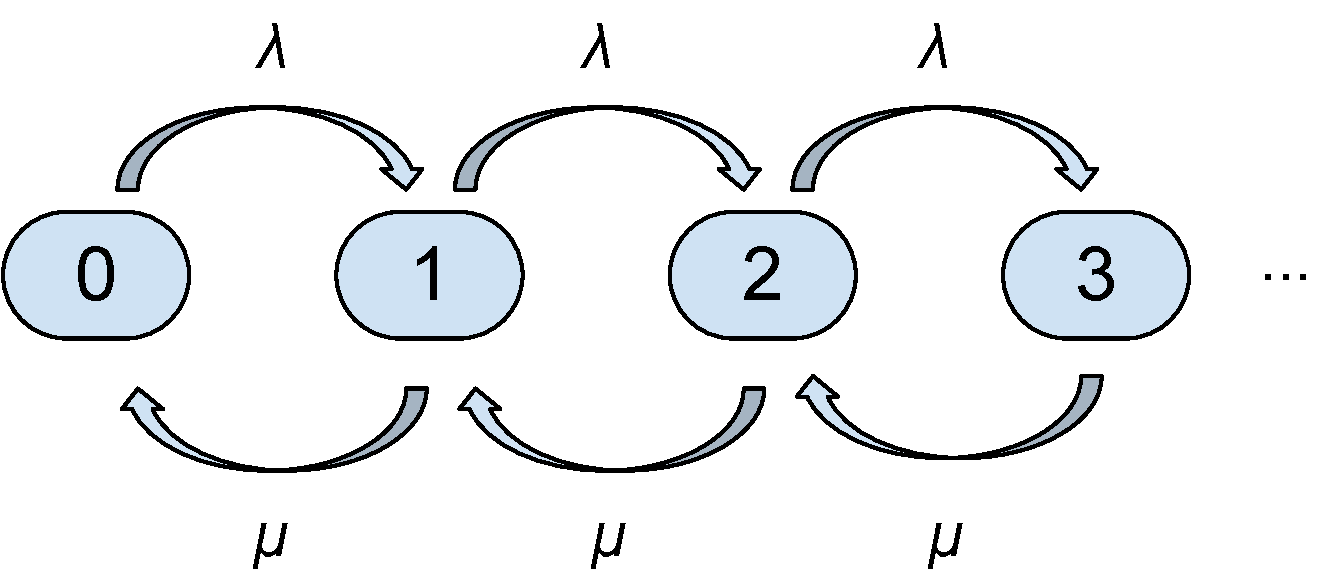
\includegraphics[width=7cm]{mm1Q.pdf}
\end{center}
We study queues as continuous Markov chains.
}

\frame{\frametitle{Stability of queues}
Recall:
\begin{center}
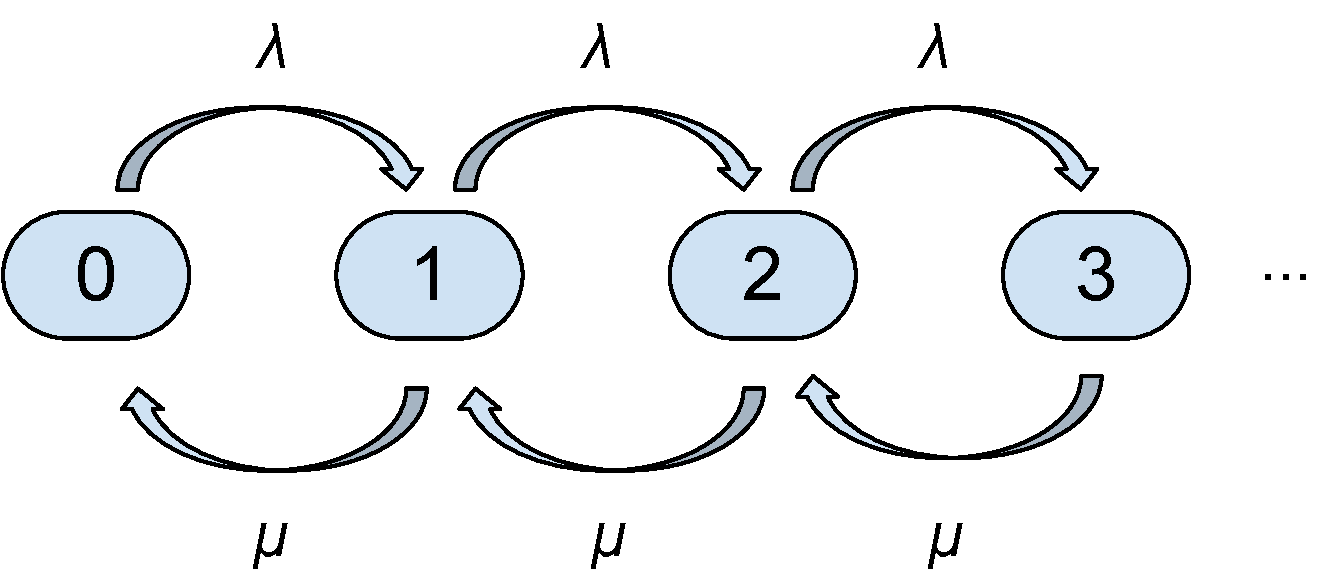
\includegraphics[width=7cm]{mm1Q.pdf}
\end{center}
This has rate matrix:
$$\begin{pmatrix}
-\lambda&\lambda&0&0&0&\dots\\
\mu&-(\lambda+\mu)&\lambda&0&0&\dots\\
0&\mu&-(\lambda+\mu)&\lambda&0&\dots\\
\vdots&\vdots&\vdots&\vdots&\vdots&\ddots
\end{pmatrix}$$
}

\frame{\frametitle{Steady state of a single server queue}
Consider a single server queue with infinite buffer, arrival rate $\lambda$ and service rate $\mu$, as shown on the previous slide.\\\vspace{.5cm}
Using the transition diagram on the previous slide, and balancing the probability flows into and out of states, the steady-state equations for this model are:
$$\begin{array}{@{}r@{\;}c@{\;}l@{}}
\pi_0\lambda&=&\pi_1\mu\\[2mm]
\pi_1(\lambda+\mu)&=&\pi_0\lambda+\pi_2\mu\\[2mm]
\pi_2(\lambda+\mu)&=&\pi_1\lambda+\pi_3\mu\\[2mm]
&\vdots&\\[2mm]
\pi_i(\lambda+\mu)&=&\pi_{i-1}\lambda+\pi_{i+1}\mu\\[2mm]
\end{array}$$
We solve these iteratively.
}

\frame{\frametitle{Steady state of a single server queue}
The first equation gives:
$$\pi_1={\lambda\over\mu}\pi_0$$
Substituting this into the second equation gives:
$$\pi_2={\lambda+\mu\over\mu}{\lambda\over\mu}\pi_0-{\lambda\over\mu}\pi_0=\left({\lambda\over\mu}\right)^2\pi_0$$
Similarly, the third equation gives: $\pi_3=\left({\lambda\over\mu}\right)^3\pi_0$. We postulate:
$$\pi_i=\left({\lambda\over\mu}\right)^i\pi_0$$
this will be proved using an inductive process.
}

\frame{\frametitle{Proof by induction}
We assume that $\pi_i=\left({\lambda\over\mu}\right)^i\pi_0$ is true for all $i\leq n$ and show that this implies that it must also hold for the $(n+1)^{th}$ term. We know:
$$\pi_i(\lambda+\mu)=\pi_{i-1}\lambda+\pi_{i+1}\mu$$
but $\pi_i=\left({\lambda\over\mu}\right)^i\pi_0$ and $\pi_{i-1}=\left({\lambda\over\mu}\right)^{i-1}\pi_0$, thus:
$$\pi_{i+1}={\lambda\over\mu}\pi_i=\left({\lambda\over\mu}\right)^{i+1}\pi_0$$
as required. We have shown that \textbf{if} the result is true for $\pi_i$ and $\pi_{i-1}$, it is true for $\pi_{i+1}$. We have also shown that it is true for $\pi_0$ and $\pi_1$, therefore it \textbf{must} be true for all $\pi_i$.
}

\frame{\frametitle{Steady state of a single server queue}
To find $\pi_0$, we use the additional equation $\sum_{i=0}^{\infty}\pi_i=1$:
$$\sum_{i=0}^{\infty}\pi_i=\sum_{i=0}^{\infty}\left({\lambda\over\mu}\right)^{i}\pi_0={\pi_0\over 1-{\lambda\over\mu}}=1$$
thus, $\pi_0=1-{\lambda\over\mu}$ and so $\pi_i=\left(1-{\lambda\over\mu}\right)\left({\lambda\over\mu}\right)^{i}$.\\\vspace{.5cm}
Note: this proof only holds for ${\lambda\over\mu}<1$ as otherwise $\sum_{i=0}^{\infty}\left({\lambda\over\mu}\right)^{i}$ does not converge. If $\lambda\geq\mu$ then the sum is infinite and there is no solution to the steady state equations. In this case the queue is \textbf{unstable}: its length grows indefinitely. (If $\lambda\geq\mu$ then customers are arriving faster than the server can deal with them.)
}

\frame{\frametitle{Steady state of a single server queue}
The \emph{traffic intensity} is given by $\rho={\lambda\over\mu}$. The $M/M/1$ queue is stable if and only if $\rho<1$.\\\vspace{.5cm}
For a stable queue, we can use the steady state distribution to describe the behaviour of the queue:
\begin{itemize}
\item The proportion of time the server is busy is $1-\pi_0=\rho$. The proportion of time the system is idle is $\pi_0$.
\item The average number of units in the system is:
$$\begin{array}{@{}r@{\;}c@{\;}l@{}}
L_c=\sum_{i=1}^{\infty}i\pi_i&=&(1-\rho)\rho\sum_{i=1}^{\infty}i\rho^{i-1}\\[2mm]
&=&(1-\rho)\rho{1\over(1-\rho)^2}\\[2mm]
&=&{\rho\over(1-\rho)}\\[2mm]
\end{array}$$
\end{itemize}
}

\frame{\frametitle{Steady state of a single server queue}
\begin{itemize}
\item The average number of units in the queue is:
$$\begin{array}{@{}r@{\;}c@{\;}l@{}}
L_q=\sum_{i=1}^{\infty}(i-1)\pi_i&=&\sum_{i=1}^{\infty}i\pi_i-\sum_{i=1}^{\infty}\pi_i\\[2mm]
&=&L_c-(1-\pi_0)\\[2mm]
&=&{\rho^2\over(1-\rho)}\\[2mm]
\end{array}$$
\end{itemize}}

\frame{\frametitle{Steady state of a single server queue}
\begin{itemize}
\item The average time in the queue $W_q$ (assuming FIFO) is the average number of units in the system when the new unit arrives ($L_c$), multipled by the average time for one unit to be served $\left({1\over \mu}\right)$. Therefore:
$$W_q={\rho\over\mu(1-\rho)}$$
\end{itemize}}

\frame{\frametitle{Steady state of a single server queue}
\begin{itemize}
\item The average time spent in the system $W_c$ (assuming FIFO) is the average spent in the queue ($W_q$) plus the average time it takes to service one unit. Therefore:
$$\begin{array}{@{}r@{\;}c@{\;}l@{}}
W_c&=&W_q+{1\over\mu}\\[2mm]
&=&{1\over\mu(1-\rho)}\\[2mm]
\end{array}$$
\end{itemize}
(note that we have used the memoryless property to tell us that when you arrive, the service time remaining for the person currently being served is still $NegExp(\lambda)$)}

\frame{\frametitle{Little's queueing formulae}
For any $G/G/m/n$ queue take:
$$
\begin{array}{@{}cc@{}}
\lambda=\text{arrivals per unit time}&\\[2mm]
L_c=\text{mean number in system}&W_c=\text{mean time in system}\\[2mm]
L_q=\text{mean number in queue}&W_q=\text{mean time in queue}\\[2mm]
L_s=\text{mean number in service}&W_s=\text{mean time in service}
\end{array}
$$
then provided the queue has a long-term steady state:
$$\begin{array}{@{}r@{\;}c@{\;}l@{}}
L_c&=&\lambda W_c\\[2mm]
L_q&=&\lambda W_q\\[2mm]
L_s&=&\lambda W_s
\end{array}$$
Note that the units match: $\lambda$ is measured in customer/time, $L$ is measured in customers and $W$ is measured in time.
}

\frame{\frametitle{Little's queueing formulae}
For any $M/M/1$ queue:
$$
\begin{array}{@{}cc@{}}
L_c={\rho\over1-\rho}&W_c={1\over\mu(1-\rho)}\\[2mm]
L_q={\rho^2\over1-\rho}&W_q={\rho\over\mu(1-\rho)}\\[2mm]
L_s=\rho&W_s={1\over\mu}
\end{array}
$$}

\section{Multi Server Markovian Queues}
\frame{\frametitle{Multi-server queues}}
\frame{\frametitle{Multi-server queues}
The $M/M/2$ queue.\\
Suppose we have arrivals at rate $\lambda$, and two servers who each serve at rate $\mu$. The operational difference between two servers rate $\mu$ each, and a single server rate $2\mu$, is that if there is only one person in the system then only one server is active at rate $\mu$.
\begin{center}
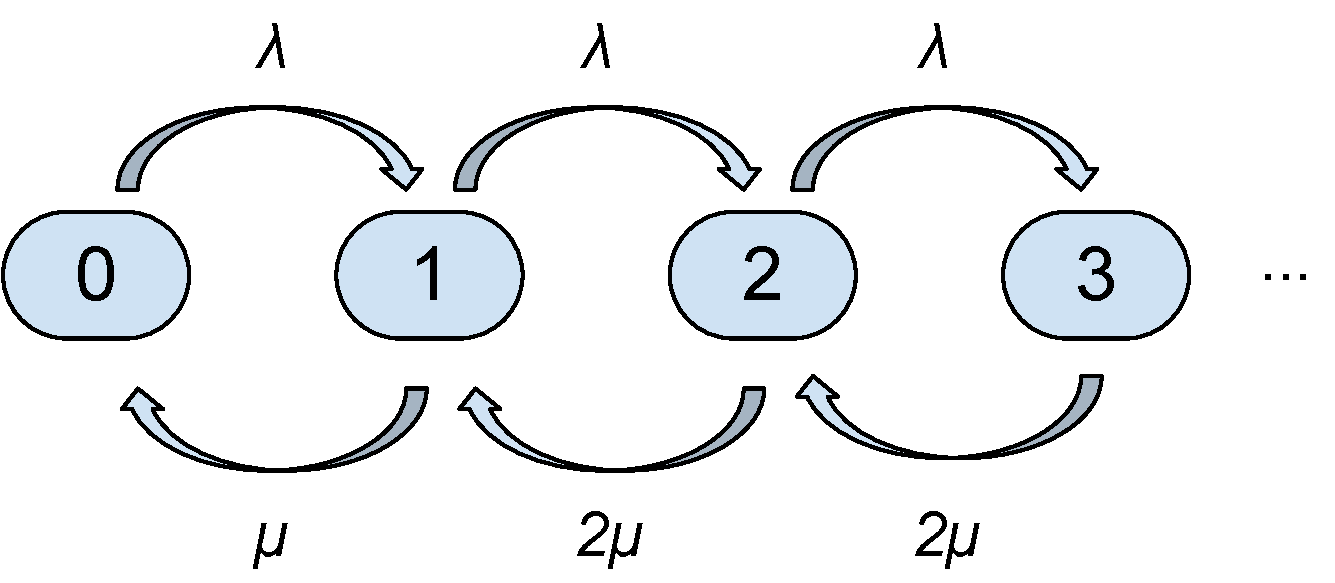
\includegraphics[width=7cm]{mm2Q.pdf}
\end{center}}

\frame{\frametitle{Multi-server queues}
The steady state equations are
$$\begin{array}{@{}r@{\;}c@{\;}l@{}}
\pi_0\lambda&=&\pi_1\mu\\[2mm]
\pi_1(\lambda+\mu)&=&\pi_0\lambda+\pi_22\mu\\[2mm]
\pi_2(\lambda+2\mu)&=&\pi_1\lambda+\pi_32\mu\\[2mm]
&\vdots&\\[2mm]
\pi_i(\lambda+2\mu)&=&\pi_{i-1}\lambda+\pi_{i+1}2\mu\\[2mm]
\end{array}$$
Solving these iteratively we obtain:
$$\pi_{i}={\lambda^i\over 2^{i-1}\mu^i}\pi_0\text{ for all }i\geq 1$$
}

\frame{\frametitle{Multi-server queues}
Setting $\sum_{i=0}^{\infty}\pi_i=1$ gives:
$$\begin{array}{@{}r@{\;}c@{\;}l@{}}
\sum_{i=0}^{\infty}\pi_i&=&\pi_0\left(1+{\lambda\over\mu}\sum_{i=1}^{\infty}{\lambda^{i-1}\over 2^{i-1}\mu^{i-1}}\right)\\[2mm]
&=&\pi_0\left(1+{\lambda\over\mu}{1\over 1-{\lambda\over2\mu}}\right)\\[2mm]
&=&1\\[2mm]
\end{array}$$
This only works if $\lambda<2\mu$, otherwise the sum does not converge and no solution exists. In this case we have $\rho={\lambda\over2\mu}$. So for $\rho<1$ we have:
$$\pi_0={1-\rho\over1+\rho}\;\;\;\;\;\pi_i=2{1-\rho\over1+\rho}\rho^i$$
}

\frame{\frametitle{Multi-server queues}
We have arrivals at a rate $\lambda$ and $k$ servers who each serve at a rate $\mu$.
\begin{center}
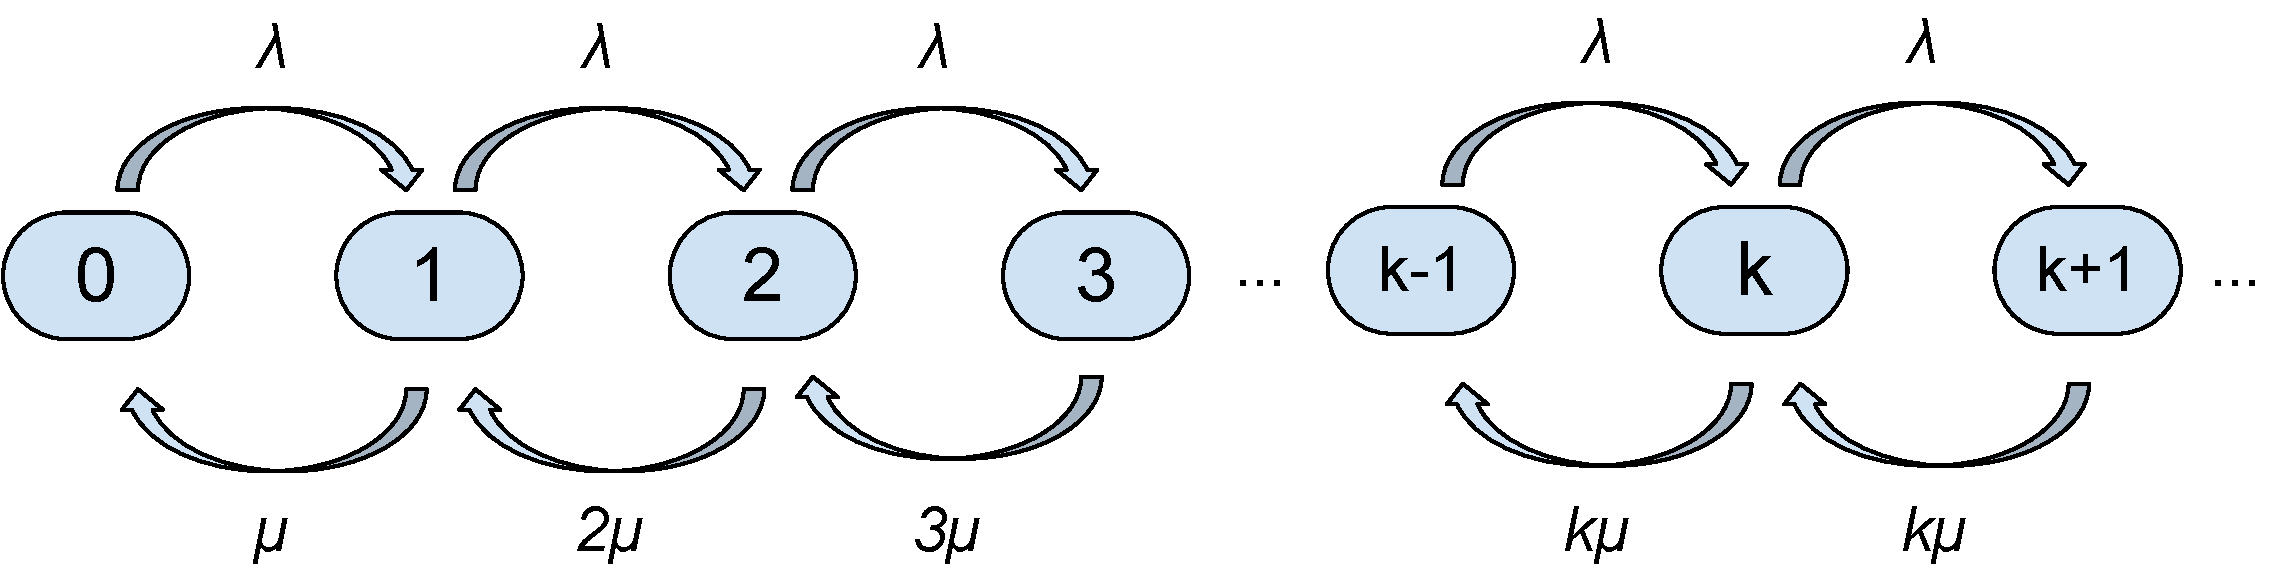
\includegraphics[width=7cm]{mmkQ.pdf}
\end{center}
}

\frame{\frametitle{Multi-server queues}
The steady state equations are
$$\begin{array}{@{}r@{\;}c@{\;}l@{}}
\pi_0\lambda&=&\pi_1\mu\\[2mm]
\pi_1(\lambda+\mu)&=&\pi_0\lambda+\pi_22\mu\\[2mm]
\pi_2(\lambda+2\mu)&=&\pi_1\lambda+\pi_33\mu\\[2mm]
&\vdots&\\[2mm]
\pi_k(\lambda+k\mu)&=&\pi_{k-1}\lambda+\pi_{k+1}k\mu\\[2mm]
&\vdots&\\[2mm]
\pi_i(\lambda+k\mu)&=&\pi_{i-1}\lambda+\pi_{i+1}k\mu\text{ for }i>k\\[2mm]
\end{array}$$
}

\frame{\frametitle{Multi-server queues}
Solving these iteratively we obtain:
$$\pi_i=\left\{\;\begin{array}{@{}c@{}}
{\left(\lambda\over\mu \right)^i\over i!}\pi_0\text{ for }i<k\\[2mm]
{\left(\lambda\over\mu \right)^i\over k!k^{i-k}}\pi_0\text{ for }i\geq k\\[2mm]
\end{array}
\right.$$
We now set $\sum_{i=0}^{\infty}\pi_i=1$ to give:
$$1=\left(\sum_{i=0}^{k-1}{\left(\lambda\over\mu \right)^i\over i!}+\sum_{i=k}^{\infty}{\left(\lambda\over\mu \right)^i\over k!k^{i-k}}\right)\pi_0$$
}

\frame{\frametitle{Multi-server queues}
Consider the second term in the sum:
$$\sum_{i=k}^{\infty}{\left(\lambda\over\mu \right)^i\over k!k^{i-k}}={1\over k!}\sum_{i=k}^{\infty}{\left(\lambda\over\mu \right)^i\over k^{i-k}}$$
Let $j=i-k$, then:
$$\begin{array}{@{}r@{\;}c@{\;}l@{}}
{1\over k!}\sum_{i=k}^{\infty}{\left(\lambda\over\mu \right)^i\over k^{i-k}}&=&{1\over k!}\sum_{j=0}^{\infty}{\left(\lambda\over\mu \right)^{j+k}\over k^{j}}\\[2mm]
&=&{\left(\lambda\over\mu \right)^{k}\over k!}\sum_{j=0}^{\infty}{\left(\lambda\over\mu \right)^{j}\over k^{j}}\\[2mm]
&=&{\left(\lambda\over\mu \right)^{k}\over k!}\sum_{j=0}^{\infty}{\left(\lambda\over k\mu \right)^j}\\[2mm]
&=&{\left(\lambda\over \mu \right)^k\over k!\left(1-{\lambda\over k\mu} \right)}\\[2mm]
\end{array}$$
}

\frame{\frametitle{Multi-server queues}
Thus:
$$\pi_0={1\over\left(\sum_{i=0}^{k-1}{\left(\lambda\over\mu\right)^i\over i!}+{\left(\lambda\over \mu \right)^k\over k!\left(1-\left(\lambda\over k\mu \right)\right)}\right)}$$}

\frame{\frametitle{Multi-server queues}
The probability an arrival will have to wait for service is the probability that all servers are busy:
$$P(\text{wait for service})=\sum_{i=k}^{\infty}\pi_i={\left(\lambda\over \mu \right)^k\over k!\left(1-\left(\lambda\over k\mu \right)\right)}\pi_0$$
The expected number of servers busy is:
$$E(\text{channels busy})=\sum_{i=1}^{k-1}i\pi_i+k\sum_{i=k}^{\infty}\pi_i={\lambda\over\mu}$$
The expected number in the queue is:
$$L_q=\sum_{i=k+1}^{\infty}(i-k)\pi_i={\left(\lambda\over \mu \right)^{k+1}\pi_0\over kk!\left(1-{\lambda\over k\mu} \right)^2}$$
}

\frame{\frametitle{Multi-server queues}
The expected number in the system is the expected number in the queue plus the expected number in service:
$$L_c=L_q+{\lambda\over\mu}$$
We can use Little's formula to find the expected time in the system $W_c$ and the queue $W_q$:
$$\begin{array}{@{}r@{\;}c@{\;}l@{}}
W_c={L_c\over\lambda}\\[2mm]
W_q={L_q\over\lambda}\\[2mm]
\end{array}
$$
}

\frame{\frametitle{Multi-server queue with finite buffer}
Consider a queue with arrival rate $\lambda,\;2$ servers each with service rate $\mu$, and a finite buffer of size 2. That is, at most 2 units can wait in the queue. Arrivals when the buffer is full are assumed to be lost to the system.\\\vspace{.5cm}
Let the state be the number of customers in the system, which thus varies from 0 to 4. The transition diagram for this system is:
\begin{center}
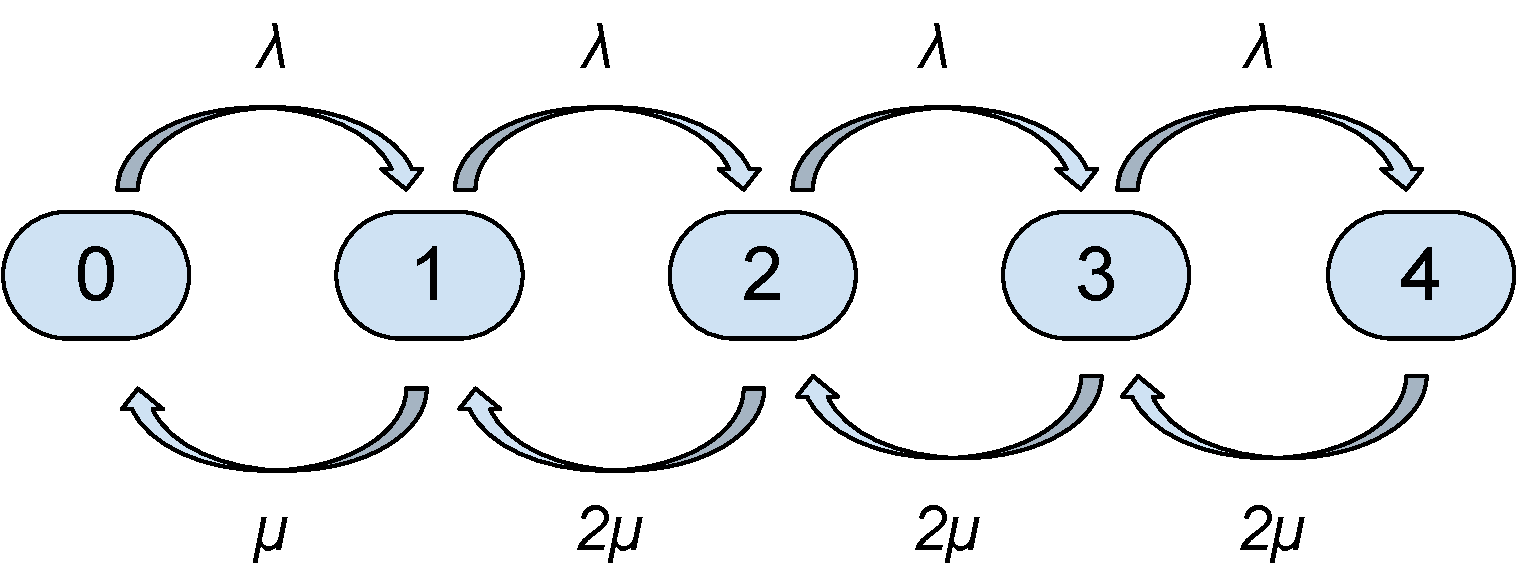
\includegraphics[width=7cm]{mm44Q.pdf}
\end{center}
}

\frame{\frametitle{Multi-server queue with finite buffer}As we have a finite buffer there are a finite number of steady-state equations:
$$\begin{array}{@{}r@{\;}c@{\;}l@{}}
\pi_0\lambda&=&\pi_1\mu\\[2mm]
\pi_1(\lambda+\mu)&=&\pi_0\lambda+\pi_22\mu\\[2mm]
\pi_2(\lambda+2\mu)&=&\pi_1\lambda+\pi_32\mu\\[2mm]
\pi_3(\lambda+2\mu)&=&\pi_2\lambda+\pi_42\mu\\[2mm]
\pi_42\mu&=&\pi_3\lambda
\end{array}
$$
Note that these equations are not independent: if you add all the equations together and cancel like terms you just get $0=0$. This is not a problem however, as we have the additional equation:
$$\pi_0+\pi_1+\pi_2+\pi_3+\pi_4=1$$
}

\frame{\frametitle{Multi-server queue with finite buffer}
Putting $\rho={\lambda\over 2\mu}$, the solution to this system is:
$$\begin{array}{@{}r@{\;}c@{\;}l@{}}
\pi_0={1-\rho\over1+\rho-2\rho^5}\\[2mm]
\pi_i=2\rho^i\pi_0\text{ for }i\geq1
\end{array}
$$
Note, in this case the steady-state equations have a solution even if $\rho\geq1$. This is possible because the finite buffer prevents the length of the queue heading off to infinity.\\\vspace{.5cm}
Exercise: use the steady state distribution to calculate the server utility, average number in the system and average time spent waiting. What happens as $\rho\to\infty$.
}

\frame{\frametitle{Machine interference model}
Consider a shop floor with $m$ machines and a single operator, whose job is to reset/repair machines when they jam or break down. Suppose that each machine breaks down at a rate $\lambda$ (average time between breakdowns is ${1\over\lambda}$), and that the operator repairs machines at rate $\mu$ (average time to repair a machine is ${1\over \mu}$).
\begin{center}
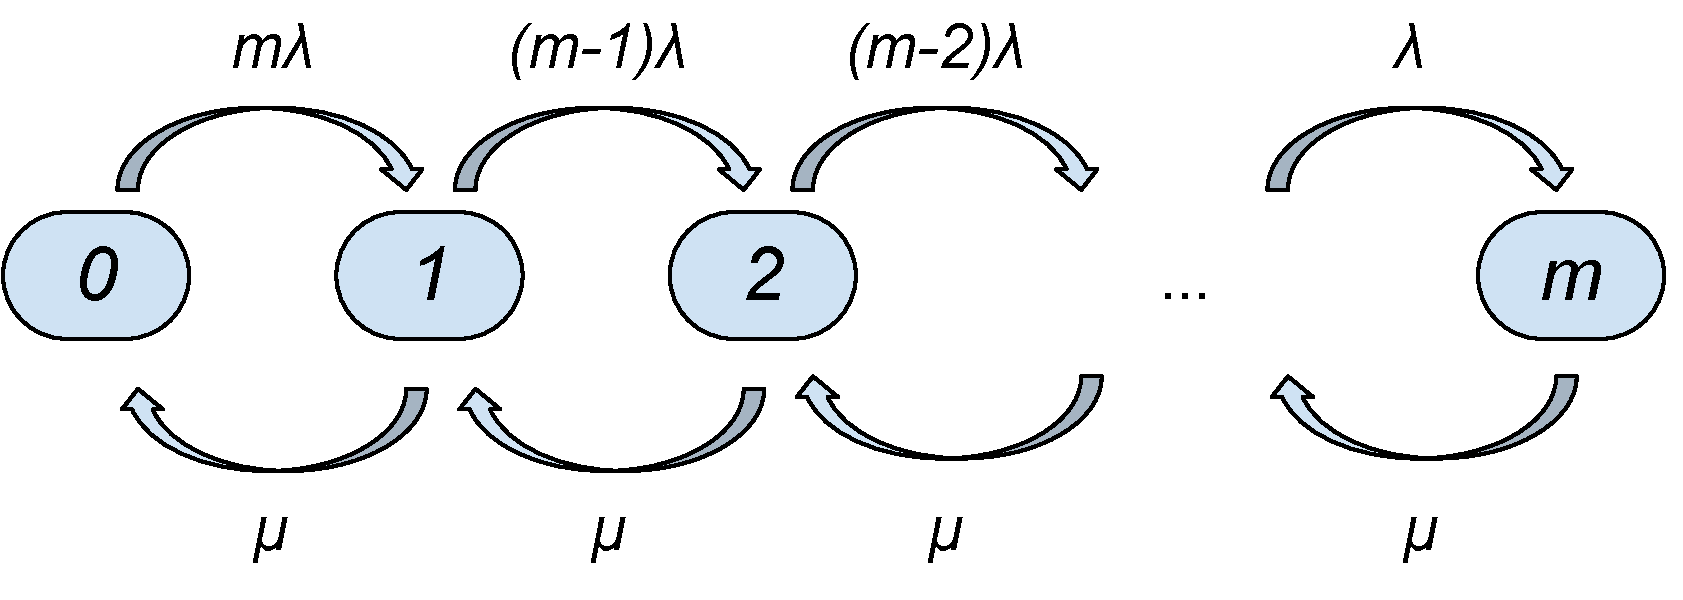
\includegraphics[width=7cm]{machine_interference_model.pdf}
\end{center}
}

\frame{\frametitle{Machine interference model}
The steady state equations:
$$\begin{array}{@{}r@{\;}c@{\;}l@{}}
\pi_0m\lambda&=&\pi_1\mu\\[2mm]
\pi_1((m-1)\lambda+\mu)&=&\pi_0m\lambda+\pi_2\mu\\[2mm]
&\vdots&\\[2mm]
\pi_{m-1}(\lambda+\mu)&=&\pi_{m-2}2\lambda+\pi_m\mu\\[2mm]
\pi_{m}\mu&=&\pi_{m-1}\lambda
\end{array}$$
The solution to these equations is:
$$\pi_i={m!\over (m-i)!}\left(\lambda\over\mu\right)^i\pi_0$$
}

\frame{\frametitle{General Birth-Death Process}
All of the examples we have seen so far can be viewed as examples of a birth-death process. If we let the state $i$ correspond to the size of population, then a transition $i\to i+1$ corresponds to a birth, and a transition $i\to i-1$ corresponds to a death. (Note that we allow transitions from $0\to1$, which correspond to immigration from a separate population.)\\\vspace{.5cm}
A general birth death process allows the birth rate and death rate to depend on the current state, i.e. we jump from $i\to i+1$ at rate $\lambda_i$, and from $i\to i-1$ at rate $\mu_i$. The transition diagram is:
\begin{center}
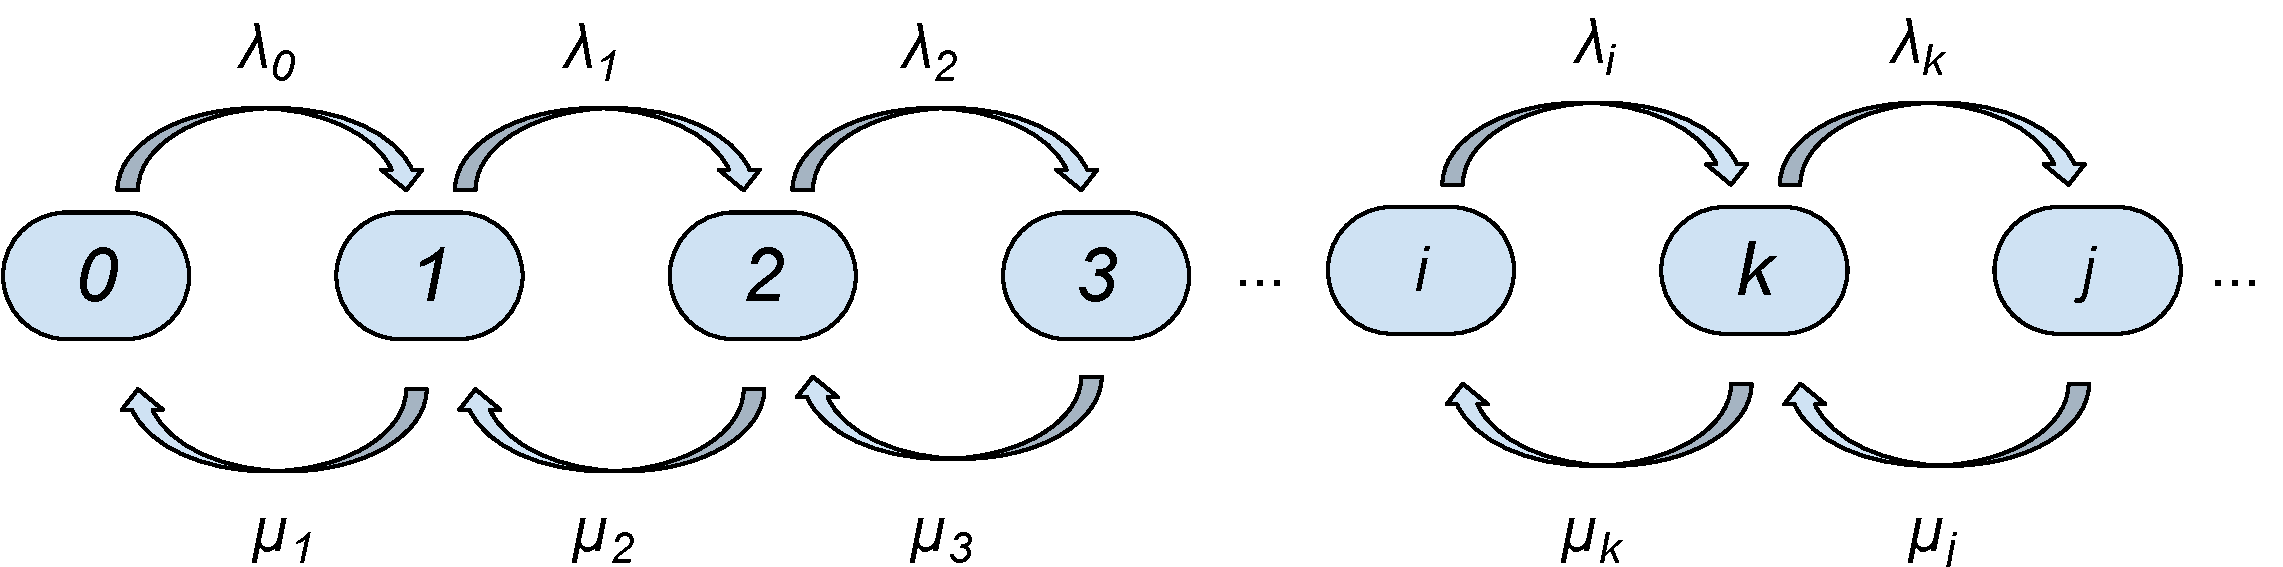
\includegraphics[width=7cm]{Generel_birth_death_process.pdf}
\end{center}
}

\frame{\frametitle{General Birth-Death Process}
The steady state equations are:
$$\begin{array}{@{}r@{\;}c@{\;}l@{}}
\pi_0\lambda_0&=&\pi_1\mu_1\\[2mm]
\pi_1(\lambda_1+\mu_1)&=&\pi_0\lambda_0+\pi_2\mu_2\\[2mm]
&\vdots&\\[2mm]
\pi_{i}(\lambda_i+\mu_i)&=&\pi_{i-1}\lambda_{i-1}+\pi_{i+1}\mu_{i+1}
\end{array}$$
The solution to these equations is, for $i\geq1$:
$$\pi_i={\lambda_0\lambda_1\dots\lambda_{i-1}\over\mu_1\mu_2\dots\mu_i}\pi_0$$
Thus, a steady-state distribution exists provided:
$$\sum_{i=1}^{\infty}{\lambda_0\lambda_1\dots\lambda_{i-1}\over\mu_1\mu_2\dots\mu_i}<\infty$$
}
\end{document}
